% \documentclass{article}
\documentclass[tikz,margin=5mm]{standalone}
\usepackage{tikz}
\begin{document}
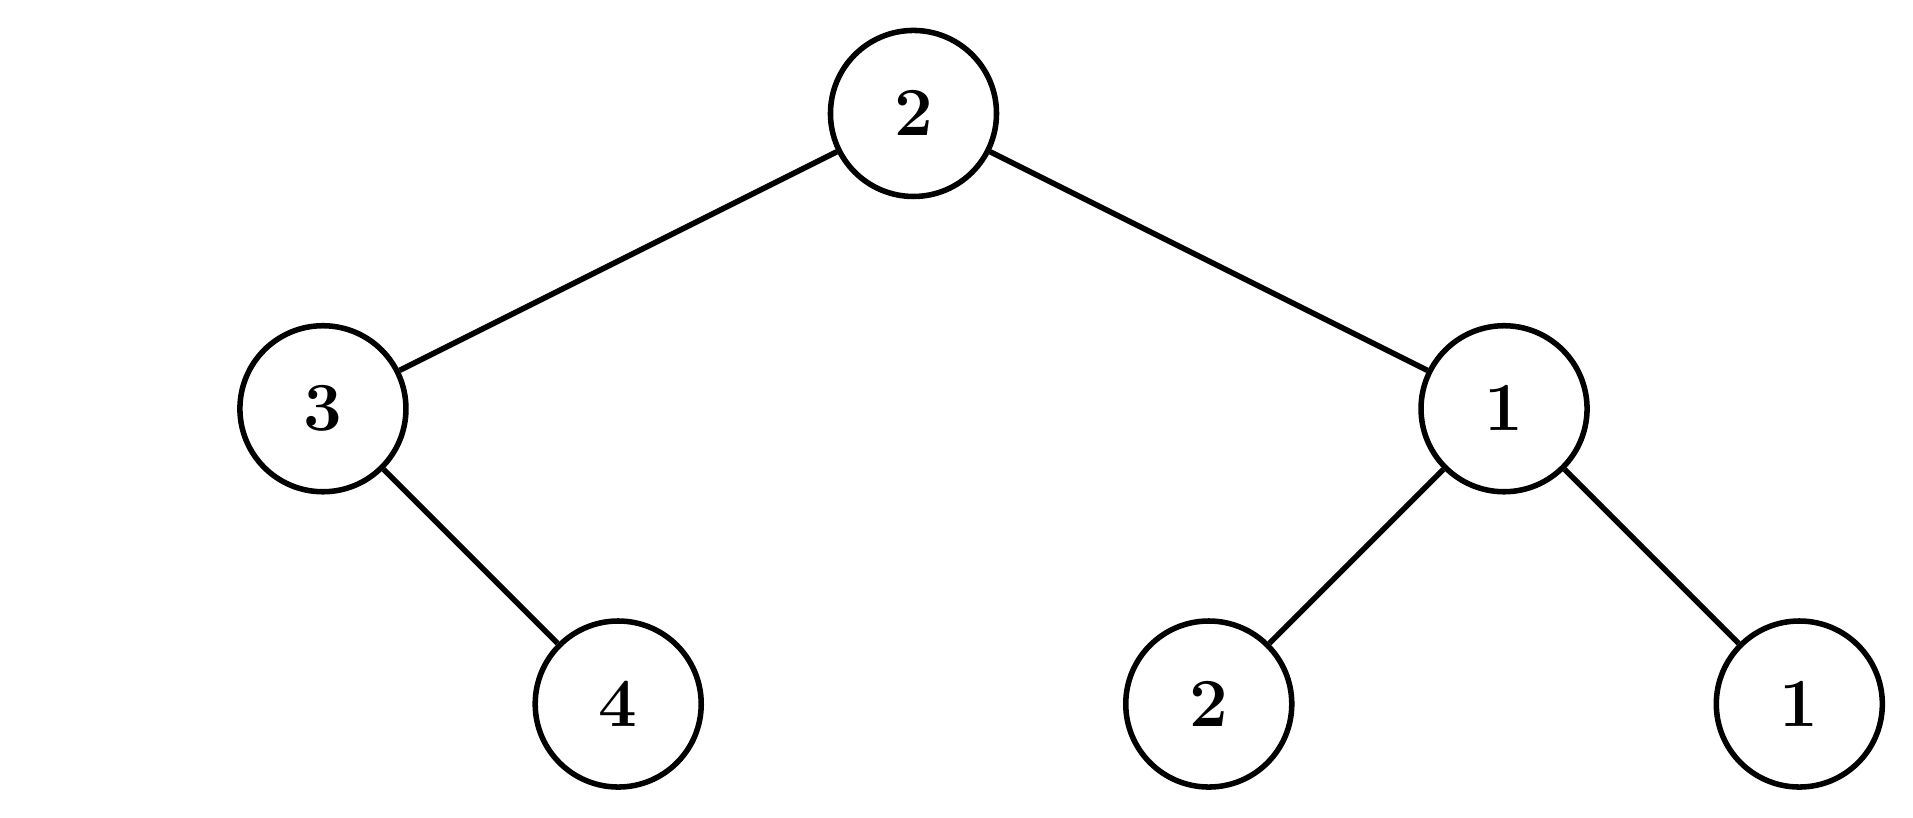
\begin{tikzpicture}[
  scale=2.5,
  every node/.style = {minimum width = 6em, draw, circle, font=\Huge\bf, line width=2pt},
  edge from parent/.style={line width=2pt, draw},
  level/.style = {sibling distance = 60mm/#1}
]
  \node {2}
  child {
        node {3} 
        child {edge from parent[draw = none]}
        child {node {4}}
        % child {node {43}
        %        child {node {36}}
        %        child {edge from parent[draw = none]}
        %       }
        }
  child {node {1}
    child {node {2}}
               %  child {edge from parent[draw = none]}
               %  child {node {83}}
               % }
        child {node {1}}
        };
\end{tikzpicture}
\end{document}

